\documentclass[a4paper, 11pt]{article}
\usepackage[utf8]{inputenc}

\usepackage[breaklinks, colorlinks=true, citecolor=black, linkcolor=blue, urlcolor=blue, filecolor=blue]{hyperref}

\usepackage{comment}

\usepackage[center, labelfont=bf]{caption}
\captionsetup{justification=justified, singlelinecheck=false} % Justify left

\usepackage{amsmath} % Math equation

% For table
\usepackage{multirow}
\usepackage[table, xcdraw]{xcolor}

% Page definitions
\setlength{\topmargin}{1.5cm}
\setlength{\headheight}{1.1\baselineskip}
\setlength{\headsep}{20pt}
\setlength{\topskip}{12pt}
\setlength{\evensidemargin}{0pt}
\setlength{\oddsidemargin}{0pt}
\setlength{\textheight}{240mm}
\setlength{\textwidth}{160mm}
\setlength{\voffset}{-2cm}
\setlength{\parindent}{0pt}
\setlength{\parskip}{6pt}

\usepackage{natbib} % Bibliography
\bibliographystyle{unsrt}

\usepackage{graphicx}
\graphicspath{ {../Figures/} }

%opening
\title{The Impact of Model Assumptions on RES Drought Analysis}
\author{Boris Morin, Damian Flynn, Aina Maimó Far, Conor Sweeney}

\begin{document}

\maketitle

\begin{abstract}


Keywords: 
\end{abstract}

\section{Introduction}

As the global shift towards renewable energy accelerates, the European Union (EU) has positioned itself as a leader in climate and energy policy. Under the revised European Green Deal \cite{greendeal2023report}, the EU has set ambitious targets to achieve at least 69\% of electricity generation from renewable energy sources (RES) by 2030. This is a significant increase from 2022, when RES accounted for over 41\% of the EU’s electricity generation \cite{europe2023stat}. Meeting this goal is a key step in reducing greenhouse gas emissions and ensuring a sustainable energy future.

However, as reliance on RES grows, so does the challenge of managing the variability of weather-dependent energy sources like wind and PhotoVoltaic (PV) power. This challenge is further intensified by the increasing electrification of energy sectors which places additional demand on the power system~\cite{bloomfield2021}. As more sectors shift from fossil fuels to electricity, the power grid becomes increasingly sensitive to meteorological conditions~\cite{bloomfield2016, vanderWiel2019drought}. In this context, periods of low renewable generation often referred to as \textit{Dunkelflaute} or RES droughts, pose a greater risk to grid stability and energy security. Ensuring a reliable electricity supply during these RES droughts is crucial for maintaining a resilient energy system capable of meeting both the growing demand for electricity and the EU’s decarbonization targets.

For this study, a RES drought event is defined when the average capacity factor (CF) remains below a fixed threshold for a given duration, following the methodology established in previous research~\cite{kaspar2019drought, ohba2022drought, mockert2023drought, mayer2023drought}. Other studies have employed varying methodologies for defining RES droughts. One approach uses relative thresholds that change over the course of the year to account for seasonal variations in renewable energy generation~\cite{raynaud2018drought, rinaldi2021drought, gangopadhyay2022drought, allen2023drought, kapica2024drought}. Another common method relies on quantile-based thresholds, where drought events are defined by identifying periods of unusually low generation relative to historical production levels, typically based on the lowest production percentiles~\cite{bracken2024drought, allen2023drought}. Additionally, some studies combine these definitions with metrics that incorporate the demand side of energy consumption, analysing the balance between supply and demand during drought periods~\cite{raynaud2018drought, rinaldi2021drought, allen2023drought, bracken2024drought}. In this paper, the focus is exclusively on energy generation, using a fixed threshold approach to define RES droughts. 

RES drought events can be identified from wind and PV CF time series. In this study, we use three different datasets, all of them driven by ERA5 data~\cite{hersbach2020era5}. The first two datasets are part of C3S Energy (C3S-E)~\cite{cds2023energy}, an energy-based operational dataset produced by the EU Copernicus Climate Change Service~\cite{dubus2023energy} (C3S). One of the C3S-E datasets provides CF time series aggregated at the national scale. Another C3S-E dataset provides the CF time series at each grid point, at the ERA5 resolution of 0.25°. The third dataset is produced by the authors using the Atlite model~\cite{hofman2021atlite}, which converts the  ERA5 atmospheric data to a generation time series using specified wind turbine and PV panel models. 

\begin{comment}
The C3S-E national dataset assumes RES farms exist at every grid point, whereas for the C3S-E Gridded and Atlite datasets, the location of each RES farm is applied. \textcolor{magenta}{Do you think you could add somehow that the C3S-E datasets assume specific wind and PV conversion models? Perhaps this should not be in the introduction, but since farms are mentioned I would include the model as well.}
\end{comment}


This study aims to quantify the occurrence of RES drought events in Ireland for two energy scenarios. The first represents the current energy mix, predominantly driven by wind, while the second is based on projected energy scenarios, featuring a more balanced share between wind and PV. A consistent methodology is used to identify RES droughts for each of the three datasets, and differences in the frequency, the duration and the seasonality are presented. 

\begin{comment}
	 \textcolor{magenta}{Did we say we are avoiding temporal references in scenarios? I get that ignoring what they represent is not the way to go but the line is very fine I would say}
\end{comment}

The datasets used in this study are detailed in section~\ref{sec:data}, which describes their sources, characteristics, and relevance for evaluating RES droughts. Section~\ref{sec:methods} outlines the energy models used to simulate wind and PV generation and provides the methodology for defining and identifying RES drought events, including the thresholds and metrics applied. In section~\ref{sec:analysis}, an in-depth analysis of RES drought occurrences is presented for the two energy scenarios, highlighting key differences across the datasets and the effects of varying energy capacities. Finally, section~\ref{sec:DiscConc} offers a discussion of the results in the context of energy reliability and future planning, followed by the main conclusions and recommendations for further research.

\section{Data}
\label{sec:data}

To construct and validate the models, this study uses publicly available datasets from EirGrid, the Republic of Ireland's transmission system operator, and the ERA5 reanalysis dataset. These datasets provide necessary inputs for estimating the CF for wind and PV energy generation.

\subsection{EirGrid}
\label{sec:eirgrid}

EirGrid provides detailed datasets for all wind and PV farms in the Republic of Ireland and Northern Ireland (collectively referred to as Ireland) from 1990 to the present~\cite{eirgrid}. These datasets include information on each farm’s installed capacity, name, and connection date. To improve these datasets, the GPS coordinates for each farm were manually determined using online search.

EirGrid also provides a wide range of energy system variables for wind (2014-present) and PV (2018-present) energy generation. For our study, we use generation which refers to the actual amount of energy produced by the wind or PV farms. This is then combined with the installed capacity to compute the CF. \textcolor{cyan}{Change}

\begin{comment}
boris: we use availability which indicates the potential energy output if the farms were operating at full capacity 
\end{comment}

\subsection{Atmospheric Variables}
\label{sec:era5}
 
Atlite and C3S-E datasets are driven by the ERA5 reanalysis dataset~\cite{hersbach2020era5}, produced by the European Centre for Medium-Range Weather Forecasts (ECMWF). This global gridded dataset provides hourly atmospheric variables from 1940 to the present. It is widely used for estimating PV and wind energy~\cite{mockert2023drought, dubus2023energy, brown2021drought, otero2022drought}. Table~\ref{tab:var_name} lists the ERA5 variables used in the models to generate the Atlite and C3S-Energy datasets.

\begin{table}[h!]
	\centering
	\begin{tabular}{|l|c|}
		\hline
		{\textbf{ERA5 name}}      & \textbf{variable} \\ \hline
		100 metre zonal and meridional wind speed   & $u_{100}$, $v_{100}$ \\
		2 metre temperature                         & $t2m$ \\
		Surface net solar radiation                 & $ssr$ \\
		Surface solar radiation downwards           & $ssrd$  \\
		Top of atmosphere incident radiation        & $tisr$  \\
		Total sky direct solar radiation at surface & $fdir$  \\ \hline
	\end{tabular}
	\caption{Variables retrieved from ERA5 dataset}
	\label{tab:var_name}
\end{table}

\subsection{C3S Energy}
\label{sec:c3se}

The Copernicus Climate Change Service (\textcolor{cyan}{I have defined C3S-E before, should I use it here ?} \textcolor{magenta}{I am not against introducing some acronyms twice, same as for some references being in the introduction and data, but I would say there is no right or wrong way necessarily} )has developed a renewable energy dataset for Europe~\cite{dubus2023energy}, using ERA5 atmospheric variables and weather-to-energy models. This dataset provides hourly CF for wind and PV energy from 1979 to the present. The data are available on the same grid as the ERA5 data, which has a horizontal resolution of 0.25°. Data are also available for download at two aggregated scales: regional (NUTS 2) and national.

The C3S-E dataset estimates wind energy using wind speeds at 100 metres ($u_{100}$, $v_{100}$) and a standard turbine model, the Vestas V136/3450, with a fixed hub height of 100 m. This choice is based on expert advice and actual trend in wind turbine installation. The PV generation model used by C3S-E uses two ERA5 variables: global horizontal irradiance (referred to here as $ssrd$) and air temperature ($t2m$). PV generation is calculated multiple times using the same model with different azimuth and tilt angles. The results are aggregated based on a statistical distribution of the module angles~\cite{saintdrenan2018solar}. \textcolor{cyan}{I added a sentence to explain the reason of the Vestas choice} \textcolor{magenta}{So, basically what they are saying is that they are looking at a realistic turbine for the future, makes sense. Not necessarily linked to the article, but I wonder how realistic this turbine choice is for other countries. We know it is not for Ireland, but I am curious about the rest of Europe}

\section{Methods}
\label{sec:methods}

In this study, we use three datasets to analyse RES droughts. Data downloaded from C3S-E are used to obtain two datasets: one based on national-level (C3S-E N), and another on grid-level (C3S-E G). The third dataset is computed using the Atlite model (Atlite).

\subsection{C3S-E N}
\label{sec:C3SEN}

For national-level analyses, we use the aggregated CF time series provided by C3S-E at two levels: Republic of Ireland (NUTS0: IE) and Northern Ireland (NUTS2: UKN0). We compute a weighted average of these, based on the installed capacity of each one, to represent the total CF of Ireland. This CF time series for Ireland is based on the underlying C3S-E assumption of RES generation at every 0.25\textdegree grid point in Ireland.

\subsection{C3S-E G}
\label{sec:C3SEG}

For the second dataset, we use the gridded dataset from C3S-E to create a CF time series which is representative of the actual RES farm distribution. Using the farms' coordinates, we identify the nearest grid point on the C3S-E grid for each farm. We retrieve the CF values from the C3S-E dataset for its corresponding grid point. We then average the CF for each farm using the installed capacity as weights. This process results in a CF time series for each renewable energy source (wind and PV), which is representative of the location of the RES farms in Ireland. 

\subsection{Atlite} 
\label{sec:atlite}

Atlite is an open-source tool developed by PyPSA~\cite{hofman2021atlite}, and is widely used for estimating wind and PV generation~\cite{mockert2023drought, li2023atlite, parzen2023atlite, ali2023comparative}. This model transforms weather data into energy data, using the locations of existing RES farms as described in C3S-E G. A key distinction between C3S-E and Atlite lies in their representation of wind turbines and PV panels.

For wind power estimation, Atlite uses the wind speed at 100 metres ($u_{100}$, $v_{100}$). We provide Atlite with a wind turbine power curve generated by Renewables.ninja: Enercon E112.4500 with 0.30w smoothing~\cite{staffell2016wake} at a hub height of 100 metres, which it uses when converting wind speed to CF.

For PV power estimation, Atlite uses four irradiance variables ($ssr$, $ssrd$, $tisr$, and $fdir$) as well as the air temperature ($t2m$). We use a single PV model~\cite{beyer2004pv}, with the Kaneka Hybrid panel option. The azimuth angle is fixed at 180\textdegree (due south) and we select the optimal tilt angle option.

\subsection{Energy Scenarios}
\label{sec:scenarios}

This study investigates wind and PV CF using three models, resulting in six CF time series with the installed capacity at the end of 2023. Additionally, we analyse the combined CF of wind and PV for each model by averaging the two sources, weighted by their capacities (6.7 GW for wind, 0.6 GW for PV). This approach gives us a total of nine CF time series for the 2023 scenario. 

Given the relatively low PV capacity in Ireland in 2023 and the projected increase by 2030 (expected to increase from 0.6 GW to 8 GW), we also explore a future scenario with higher PV capacity. We generate additional CF time series reflecting the projected PV capacity in 2030 for both the Atlite and C3S-E G models, based on a roadmap published by EirGrid~\cite{eirgrid2023future}.

The wind capacity is projected to increase to 9 GW in 2030, however as the spatial distribution is not expected to significantly change we use the same CF time series. The combination of wind and PV CF is calculated once again using the new PV time series, and by averaging with the future projected capacities of RES farms. In total, we evaluate fourteen CF time series across different scenarios and models, as summarised in Table~\ref{tab:datasets}.

\begin{table}[h!]
	\centering
	\begin{tabular}{l|ccc|ccc|}
		\cline{2-7}
		& \multicolumn{3}{c|}{\textbf{Current}}                                   & \multicolumn{3}{c|}{\textbf{Projected}}                                   \\ \cline{2-7} 
	    & \multicolumn{1}{c|}{Atlite} & \multicolumn{1}{c|}{C3S-E G} & C3S-E N & \multicolumn{1}{c|}{Atlite} & \multicolumn{1}{c|}{C3S-E G} & C3S-E N \\ \hline
		\multicolumn{1}{|l|}{\textbf{PV}}      & \multicolumn{1}{c|}{x}      & \multicolumn{1}{c|}{x}       & x       & \multicolumn{1}{c|}{x}      & \multicolumn{1}{c|}{x}       &         \\
		\multicolumn{1}{|l|}{\textbf{Wind}}    & \multicolumn{1}{c|}{x}      & \multicolumn{1}{c|}{x}       & x       & \multicolumn{1}{c|}{}       & \multicolumn{1}{c|}{}        &         \\
		\multicolumn{1}{|l|}{\textbf{Combine}} & \multicolumn{1}{c|}{x}      & \multicolumn{1}{c|}{x}       & x       & \multicolumn{1}{c|}{x}      & \multicolumn{1}{c|}{x}       & x       \\ \hline
	\end{tabular}
	\caption{Summary of the time series compared in this study}
	\label{tab:datasets}
\end{table}

\subsection{RES drought definition}
\label{sec:res_drought}

In this study, we define a RES drought event as occurring when the 24-hour moving average of CF remains below a fixed threshold of 0.1 for a period of longer than 24 hours. Using the moving average captures fewer, but longer-lasting events than using the regular time series.

\begin{figure}[ht!]
	\centering
	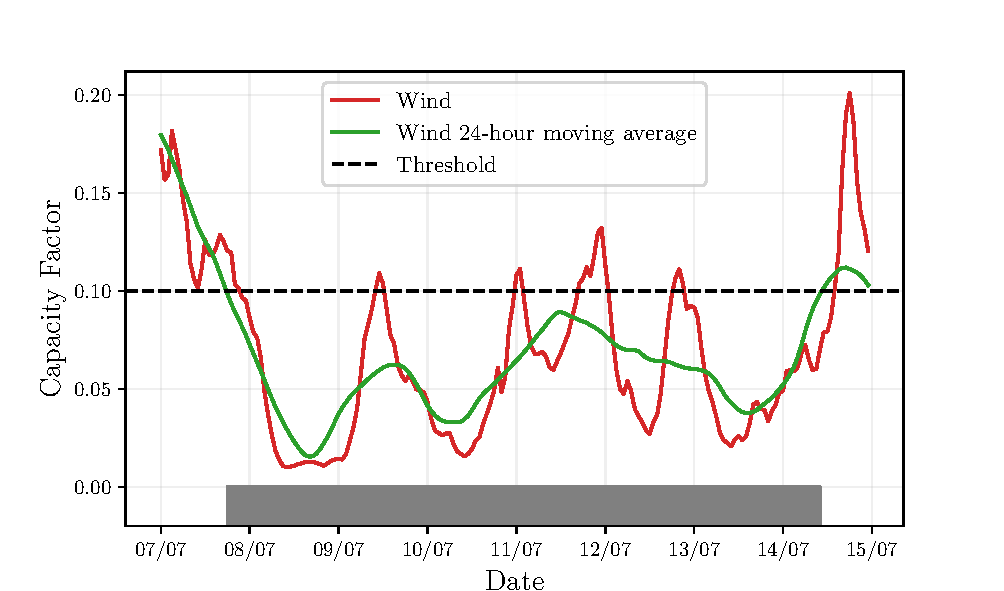
\includegraphics[width=\textwidth]{data_methods/find_res_droughts}
	\caption{Time series of CF (red) and its 24-hour moving average (green) from the 7th to the 15th of July 2021. CF threshold (dashed black). The grey bar shows the period identified as a wind drought.}
	\label{fig:find_res_droughts}
\end{figure}

Fig.~\ref{fig:find_res_droughts} illustrates the moving average  identification method. When using the moving average method, this CF time series results in one event being identified, which lasts 161 hours. In contrast, using the regular CF series would have resulted in three separate events being identified, with durations of 36, 35, and 40 hours.

\section{Results}
\label{sec:results}

\subsection{Verification}
\label{sec:verification}

Before going into the analysis of RES droughts, it is important to first verify the accuracy of the datasets used in this study. For the verification process, we use time-varying values of installed capacity to account for changes in RES development over the verification period. This step allows us to assess how well the datasets represent the production of renewable energy by comparing them against observed data.
	
\subsubsection{Wind}
\label{sec:wind_verification}

The C3S-E datasets use the Vestas V136/3450 wind turbine power curve, (Fig.~\ref{fig:power_curve} a). The Atlite model allows the user to specify the power curve. We considered the 121 power curves available for download from Renewables.ninja~\cite{staffell2016wake}. For each power curve, Renewables.ninja also provide four associated smoothed power curves. The smoothing is done by using a Gaussian filter with different standard deviations that depend on the wind speed. We generated a wind CF time series for Ireland for each of these wind turbine power curve options. The performance of each wind turbine power curve was calculated based on four skill scores: correlation coefficient (CC), root mean square error (RMSE), mean bias error (MBE), and area under the curve. The area under the curve was calculated from histograms of the hourly CF values for the most recent decade, 2014-2023. Based on these metrics, the most representative power curve for Ireland was the Enercon E112.4500 power curve with the $0.3w$ filter.

\begin{figure}[!ht]
	\centering
	\includegraphics[width=\textwidth]{verification/power_curve}
	\caption{a/ Power curves of the Enercon E112.4500 with a 0.3 filter used by Atlite (blue) and the Vestas V136/3450 used by C3S-E (orange) b/ Histograms of wind CF for Ireland from Atlite (blue), C3S-E (orange) and EirGrid (shaded)}
	\label{fig:power_curve}
\end{figure}

The smoothing of the wind turbine power curve represents the wake effect, which is important when modelling wind energy on larger scales. The histogram in Fig.~\ref{fig:power_curve}b shows that the C3S-E power curve tends to underestimate low CF values and overestimate higher ones, whereas the smoothed Atlite power curve more closely follows the recorded wind data from EirGrid.

\begin{table}[!ht]
	\centering
	\begin{tabular}{l|lll|}
		\cline{2-4}
		& \textbf{Atlite} & \textbf{C3S-E G} & \textbf{C3S-E N} \\ \hline
		\multicolumn{1}{|l|}{\textbf{CC}}   & 0.981           & 0.972            & 0.970            \\ \hline
		\multicolumn{1}{|l|}{\textbf{RMSE}} & 0.045           & 0.177            & 0.162            \\ \hline
		\multicolumn{1}{|l|}{\textbf{MBE}}   & -0.003          & 0.137            & 0.121            \\ \hline
	\end{tabular}
	\caption{Skill scores for wind for the three datasets compared to EirGrid data}
	\label{tab:wind_skill_scores}
\end{table}

The effect of the differences in the power curves are also visible in Fig.~\ref{fig:wind_verification_contour} where the Atlite model shows good agreement with the EirGrid data. In contrast, the two C3S-E datasets tend to overestimate the EirGrid CF. This is confirmed by Table~\ref{tab:wind_skill_scores}, which shows that Atlite performs better than the C3S-E datasets for all three skill scores.

\begin{figure}[!ht]
	\centering
	\includegraphics[width=\textwidth]{verification/wind_verification_contour}
	\caption{Wind CF density plot of the observed EirGrid CF (vertical axes) and modelled (horizontal axes) CF data for the Atlite  (left panel), C3S-E G (central panel) and C3S-E N (right panel) models}
	\label{fig:wind_verification_contour}
\end{figure}

Fig.~\ref{fig:bar_number_events_verification_wind} presents results for the average annual number of wind drought events during the 2014 to 2023 validation period. The figure shows that Atlite shows the best agreement overall with the observed frequency and duration of wind drought events.

\begin{figure}[!ht]
	\centering
	\includegraphics[width=\textwidth]{verification/bar_number_events_verification_wind}
	\caption{Average annual number of wind drought events for EirGrid (black), Atlite (red), C3S-E G (blue), and C3S-E N (purple) / Change plot}
	\label{fig:bar_number_events_verification_wind}
\end{figure}

\subsubsection{PV}
\label{sec:pv_verification}

The C3S-E datasets calculate PV generation multiple times using the same model with varying azimuth and tilt angles. The results are then aggregated based on a statistical distribution of module angles. Similarly to the wind CF verification, the Atlite model allows the user to select from one of three different PV panel characteristics. Following the same methodology as in the previous section, we compare the three available models using four skill scores (CC, RMSE, MB, and area under the curve). Based on the best-performing metrics, we selected the Breyer PV panel model \cite{beyer2004pv}, specifically using the Kaneka Hybrid panel option.

Figure \ref{fig:solar_verification_contour} shows that the three datasets have similar correlation when compared to the EirGrid data, which is further supported by the results shown in Table~\ref{tab:pv_skill_scores}.

\begin{table}[!ht]
	\centering
	\begin{tabular}{l|lll|}
	\cline{2-4}
	& \textbf{Atlite} & \textbf{C3S-E G} & \textbf{C3S-E N} \\ \hline
	\multicolumn{1}{|l|}{\textbf{CC}}   & 0.921           & 0.931            & 0.913            \\ \hline
	\multicolumn{1}{|l|}{\textbf{RMSE}} & 0.070           & 0.065            & 0.100            \\ \hline
	\multicolumn{1}{|l|}{\textbf{MBE}}   & 0.002           & -0.012           & -0.013           \\ \hline
	\end{tabular}
	\caption{Skill scores for wind CF for the three datasets compared to EirGrid data}
	\label{tab:pv_skill_scores}
\end{table}

\begin{figure}[h!]
	\centering
	\includegraphics[width=\textwidth]{verification/solar_verification_contour}
	\caption{PV 2D density plot of the observed EirGrid (vertical axes) and modelled (horizontal axes) CF series for the Atlite  (left panel), C3S-E G (central panel) and C3S-E N (right panel) models}	
	\label{fig:solar_verification_contour}
\end{figure}

Fig.~\ref{fig:bar_number_events_verification_pv} shows results for PV drought events. The figure reveals a lack of significant agreement between the three datasets and the EirGrid data. The main challenge in validating PV stems from the recent installation of a large proportion of the PV installed capacity in Ireland. PV Generation data suffers from large uncertainties for the first few months after each PV farm is connected, making it difficult to know what the actual CF for PV was. Given that PV farms installed in 2023 represent more than 60\% of the total capacity, this significantly impacts our ability to perform vigorous verification for PV.

\begin{figure}[!ht]
	\centering
	\includegraphics[width=\textwidth]{verification/bar_number_events_verification_pv}
	\caption{Average number of PV drought events for EirGrid (black), Atlite (red), C3S-E G (blue), and C3S-E N (purple)}
	\label{fig:bar_number_events_verification_pv}
\end{figure}


\newpage
\subsection{Analysis}
\label{sec:analysis}

In this section, we evaluate RES drought events under two different scenarios with fixed installed capacities: the current scenario, with 89\% of wind capacity(6.7 GW) and 11\% of PV capacity (0.6 GW), and a projected scenario for 2030, where wind capacity comprises 53\% (9 GW) and PV capacity increases to 47\% (8 GW). Both scenarios are driven by 45 years of ERA5 data. Using the RES drought identification process described earlier (Section~\ref{sec:res_drought}), we first analyse wind and PV droughts separately before presenting the results for combined (wind + PV) RES droughts.

\subsubsection{Annual Number of RES Droughts}

The first part of our analysis examines the annual number of RES drought events for each of the three datasets. For wind results (Fig.~\ref{fig:boxplot_number_events}a), the number of events decreases as the duration range increases, with very few events lasting longer than seven days. For PV results (Fig.~\ref{fig:boxplot_number_events}b), the number of events also declines as the duration range extends from one to eight days, followed by a slight increase for longer durations. Comparing wind and PV results (Fig.~\ref{fig:boxplot_number_events}a \& Fig.~\ref{fig:boxplot_number_events}b), the median, first, and third quartiles for PV are consistently higher or equal than those for wind, regardless of duration range or dataset. 

The bottom panels show the combination of wind and PV using two different capacity scenarios. With the current RES installation (Fig.~\ref{fig:boxplot_number_events}c), the identified RES droughts are similar to those for wind alone, as expected, due to the dominance of installed wind generation. However, in the projected scenario (Fig.~\ref{fig:boxplot_number_events}d), there is a distinct reduction in the number of events across all datasets and durations (26\% for Atlite, 20\% for C3S-E G, 18\% for C3S-E N).

The median, first, and third quartiles for the Atlite dataset are consistently greater than or equal to those of the other two datasets, regardless of the duration range or type of renewable energy considered.

\begin{figure}[!ht]
	\centering
	\includegraphics[width=\textwidth]{number_events/boxplot_number_events}
	\caption{Annual number of RES droughts for a)~Wind, b)~PV, and the combination for the c)~current and d)~projected installed capacity for Atlite (red), C3S-E G (blue), and C3S-E N (purple). The x-axis represents duration ranges in days (lower bound included), while the y-axis indicates the annual number of events. The boxes display the first and third quartiles and the median is marked by a black line. The whiskers indicate the 5th and 95th percentiles}
	\label{fig:boxplot_number_events}	
\end{figure}

\newpage
\subsubsection{Return Periods of RES Drought Duration}

The RES drought events identified over the 45 year period were used to calculate the return periods for different RES drought durations.

For wind (Fig.~\ref{fig:return_periods}a), the duration of RES droughts increases in a log-linear fashion across the three datasets. 

For PV (Fig.~\ref{fig:return_periods}b), the duration of RES droughts follows a log-linear increase for events lasting less than 16 days. Beyond this threshold, there is a sharp rise in RES drought duration for events up to a one-year return period. This sudden jump reflects the effect of winter on PV generation in Ireland, as PV generation does not exceed the CF threshold for a large part of winter. The jump for the Atlite dataset is not as large as that for the two C3S-E datasets, due to differences between the datasets in PV generation around this critical 0.1 CF threshold during winter. After this jump, the increase in drought duration continues linearly relative to the log of time. 

Similar to Fig.~\ref{fig:boxplot_number_events}c, the current installed capacity combination (Fig.~\ref{fig:return_periods}c), shows comparable results as the wind panel (Fig.~\ref{fig:return_periods}a). In the projected scenario (Fig.~\ref{fig:return_periods}d) the return periods for RES droughts increase across all durations. For example, the return period for a five-day event increases from around half a year to 21 months in the Atlite dataset, and from around a year and a half to almost three years for the two C3S-E datasets.

Across Fig.~\ref{fig:return_periods}a,~c,~d, the return periods for the Atlite dataset are consistently higher than those for the two C3S-E datasets. For example, in Fig.~\ref{fig:return_periods}c, an one-year event lasts for six months according to Atlite, but only five according to the two C3S-E datasets. Additionally, in all four panels, the results for the two C3S-E datasets are closer to each other than they are to Atlite.

\begin{figure}[!ht]
	\centering
	\includegraphics[width=0.9\textwidth]{return_periods/return_periods}
	\caption{Return periods of the duration of RES droughts for a)~Wind, b)~PV, and the combination for the c)~current and d)~projected installed capacity, for Atlite (red), C3S-E G (blue), and C3S-E N (purple). The x-axis represents the return period time in a log-scale and the y-axis indicates the duration of RES drought associated with it}
	\label{fig:return_periods}
\end{figure}

\newpage
\subsubsection{Seasonal Distribution of RES Droughts}

The seasonality of RES droughts is analysed by comparing the percentage of hours in a month identified as a RES drought. For wind (Fig.~\ref{fig:res_droughts_seasonality}a), the drought percentages are higher during the summer than in winter. For Atlite, during summer (JJA), there are on average 24\% of hours which are considered as RES drought, and only 4\% during winter (DJF). In contrast the results for PV (Fig.~\ref{fig:res_droughts_seasonality}b)  show a higher percentage in winter, with RES droughts occurring  over 60\% of the time regardless of the dataset. The Atlite results show a higher percentage of RES drought hours for wind, and a slightly lower percentage for PV, compared to the two C3S-E datasets. 

Similar to previous results, the current installed capacity wind-PV combination (Fig.~\ref{fig:res_droughts_seasonality}c), shows comparable results to the wind panel (Fig.~\ref{fig:res_droughts_seasonality}a). There is a reduction in RES drought frequency for all three datasets when looking at the projected scenario (Fig.~\ref{fig:res_droughts_seasonality}d). The reduction is greatest during the summer months, which reduces the overall seasonality. Annual reductions in the median values are from 14 to 9\% for Atlite, from 8 to 6\% for C3S-E~G, and 10 to 7\% for C3S-E~N.
 
\begin{figure}[!ht]
	\centering
	\includegraphics[width=\textwidth]{seasonality/percentage_time_events}
	\caption{Percentage of hours in a month identified as a RES drought for a)~Wind, b)~PV, and the combination for the c)~current and d)~projected installed capacity, for Atlite (red), C3S-E G (blue), and C3S-E N (purple). The x-axis represents the month of the year, and the y-axis indicates the percentage of hours. Lines correspond to the median values and the area between the first and third quartiles is shaded.}
	\label{fig:res_droughts_seasonality}
\end{figure}

\newpage
\subsubsection{Change of Threshold}

In this study, we have considered a threshold of 0.1 in CF to identify a RES drought. In order to check how the results may dependent on this threshold, we have calculated the annual number of events across a range of threshold CF values (Fig~\ref{fig:number_days_threshold}).

The results for wind (Fig.~\ref{fig:number_days_threshold}a) show an increase of number events when the threshold increases. For PV (Fig.~\ref{fig:number_days_threshold}b), the number of events first increases and then start decreasing, as smaller events are continuously merging with each other to produce a smaller number of loner events. For the current (\ref{fig:number_days_threshold}c) and projected (\ref{fig:number_days_threshold}d) installed capacity scenario, the annual number of events increase with the threshold used.

Overall, the four panels show that regardless of the threshold used, the number of events identified by Atlite is consistently higher than those identified by the two C3S-E datasets.

\begin{figure}[!ht]
	\centering
	\includegraphics[width=\textwidth]{multiple_th/number_days_threshold}
	\caption{Number of RES drought per year for a)~Wind, b)~PV, and the combination for the c)~current and d)~projected installed capacity, for Atlite (red), C3S-E G (blue), and C3S-E N (purple). The x-axis represent the threshold from 0.05 to 0.2 of the CF with a 0.01 increment. The y-axis indicates the annual number of events. Each line correspond to the median value and the first and third quartiles are shown in shaded area}
	\label{fig:number_days_threshold}
\end{figure}

\newpage
\section{Discussion and Conclusions}
\label{sec:DiscConc}

\begin{itemize}
	\item Remind differences between three datasets
	\begin{itemize}
		\item Atlite and C3S-E G: incorporate locations of RES farms
		\item Atlite models better follows EirGrid data (for Wind)
	\end{itemize}
	\item Point Arguments with examples from the figures
	\begin{itemize}
		\item The two C3S-E datasets show similar results
		\item Atlite stands out of these two datasets
	\end{itemize}
	\item Conclusion: Location of RES farms has less impact than the accuracy of modelling the CF!
	\\
	\item Impact of the 2030 scenario (Anti correlation between wind and PV) | Seasonality
	\\
	\item Risk for policymakers. The more accurate Atlite model produces more RES drought events and longer RES drought durations, an important consideration for risk-adverse decision making.
	\\
	\item Where to go next ?
	\begin{itemize}
		\item Looking at future climate data (Combine Climate and Energy scenarios)
		\item Studying broader region (Europe), which is more relevant as everything will be interconnected but more difficult as we will need to repeat verification for all EU countries
	\end{itemize}
\end{itemize}

\begin{comment}
This study has highlighted the key differences between the three datasets: Atlite, C3S-E G, and C3S-E N in their ability to model RES droughts. One of the most significant differences is how each dataset incorporates the specific locations of RES farms. Both Atlite and C3S-E G take into account the exact locations of wind and PV farms, which should, in theory, provide a more accurate representation of RES generation. However, our analysis shows that the Atlite dataset generally performs better, particularly in its wind generation estimates, where it closely follows the EirGrid data. This suggests that while the inclusion of RES farm locations is important, the accuracy of the CF modeling used by Atlite may be the determining factor in its superior performance.

When analysing the results, we found that the two C3S-E datasets (C3S-E G and C3S-E N) consistently show similar outcomes across various figures (Fig.~\ref{fig:boxplot_number_events},~\ref{fig:return_periods},~\ref{fig:res_droughts_seasonality}), suggesting that their differences in methodology have minimal impact on the results. In contrast, Atlite stands out, in its ability to model wind generation, as evidenced by the more accurate correlation with EirGrid data seen in the verification process (Section \ref{sec:wind_verification}). This distinction is further underscored in the figures, where Atlite often reports higher or more accurate return periods and a greater number of RES droughts (Fig.~\ref{fig:boxplot_number_events},~\ref{fig:return_periods}), particularly in scenarios with increased PV capacity.

One of the most critical conclusions of this study is that the specific locations of RES farms, while important, have less impact on the accuracy of RES drought modeling than the precision of the CF models themselves. Atlite's superior performance suggests that refining these models could lead to better forecasting and planning for RES droughts, which is crucial for energy security.

Looking ahead to the projected scenario, our analysis suggests a significant shift in the dynamics of RES droughts due to the anti-correlation between wind and PV generation. This scenario reveals the importance of seasonality in RES droughts (Fig.~\ref{fig:res_droughts_seasonality}), where a diversified energy portfolio that includes both wind and PV could decrease the frequency and duration of RES droughts.

For policymakers, the findings of this study highlight the risks of inadequate modeling and planning. Accurate RES drought forecasting is essential for ensuring energy security, especially as Ireland moves toward an ambitious renewable energy target.

In terms of future research, there are two main topics to explore. First, integrating future climate data with energy scenarios to better understand how climate change might affect RES droughts. Second, expanding the scope of the study to include Europe, would provide a more comprehensive understanding of RES drought in an interconnected energy grid. However, this expansion would require extensive verification across all EU countries, making it a more complex but highly relevant challenge.

\end{comment}

\newpage
\section{Acknowledgment}
Using the Climate Data Store. Thank EirGrid for the data and add a reference to the funding project or projects

\section{Funding information}

\section{Author contribution}

\bibliography{litrev}

\newpage
\section*{Appendix}

\begin{figure}[!ht]
	\centering
	\includegraphics[width=0.7\textwidth]{data_methods/farm_location_wind_pv}
	\caption{Wind and PV Farms Location in Ireland. The capacity of a farm is illustrated by the size of the dot, the year of installation is represented by its color}	
	\label{fig:farm_location_wind_pv}
\end{figure}

Figure  

\begin{table}[!ht]
	\centering
	\begin{tabular}{l|cc|l|}
		\cline{2-4}
		& \textbf{Wind} & \textbf{PV} & \textbf{Total} \\ \hline
		\multicolumn{1}{|l|}{\textbf{Republic of Ireland}} & 4,730         & 445         & 5,175          \\
		\multicolumn{1}{|l|}{\textbf{Northern Ireland}}    & 1,364         & 183         & 1,547          \\ \hline
		\multicolumn{1}{|l|}{\textbf{Total}} & \multicolumn{1}{l}{6,094} & \multicolumn{1}{l|}{628} & \textbf{6,712} \\ \hline
	\end{tabular}
	\caption{Installed Capacities of wind and PV farms (MW) as of January 2024! To be modified !}
	\label{tab:installed_capacities}
\end{table}

Figure 

\begin{figure}[!ht]
	\centering
	\includegraphics[width=0.9\textwidth]{data_methods/pv_wind_capacity_time}
	\caption{Installed capacity in Ireland}
	\label{fig:pv_wind_capacity_time}
\end{figure}



\end{document}
